\documentclass[11pt,oneside,a4paper,final]{article}

\usepackage{ifpdf}

\usepackage{fancyhdr}
\usepackage{lastpage}

\pagestyle{fancy}

\renewcommand{\headrulewidth}{0.0pt}

\lhead{}
\chead{}
\rhead{}
\lfoot{}
\cfoot{Page {\thepage} of \pageref{LastPage}}
\rfoot{}

\usepackage{longtable}

\usepackage[T1]{fontenc}  
\usepackage{textcomp}  
\usepackage{lmodern}  

% \usepackage[style=numeric,backend=biber]{biblatex}
% \usepackage[style=numeric]{biblatex}
\bibliography{programmer_guide}
\usepackage[hidelinks=true]{hyperref}
\usepackage[paper=a4paper,margin=1.6cm]{geometry}	% 1 inch margins all around
\usepackage[british=nohyphenation]{hyphsubst}
\usepackage[british]{babel}
\usepackage{graphicx}
\usepackage[font=normalsize,labelfont=sf,textfont=sf]{subfig}
\captionsetup*[subfigure]{position=bottom}
\usepackage{color}

\definecolor{mygreen}{rgb}{0,0.6,0}
\definecolor{mygray}{rgb}{0.5,0.5,0.5}
\definecolor{mymauve}{rgb}{0.58,0,0.82}

\usepackage{listings}
 \lstset{ %
  literate={"}{\textquotedbl}1,
  backgroundcolor=\color{white},   % choose the background color; you must add \usepackage{color} or \usepackage{xcolor}
  basicstyle=\footnotesize,        % the size of the fonts that are used for the code
  breakatwhitespace=false,         % sets if automatic breaks should only happen at whitespace
  breaklines=true,                 % sets automatic line breaking
  captionpos=b,                    % sets the caption-position to bottom
  commentstyle=\color{mygreen},    % comment style
%   deletekeywords={...},            % if you want to delete keywords from the given language
%   escapeinside={\%*}{*)},          % if you want to add LaTeX within your code
  extendedchars=true,              % lets you use non-ASCII characters; for 8-bits encodings only, does not work with UTF-8
  frame=single,                    % adds a frame around the code
  keepspaces=true,                 % keeps spaces in text, useful for keeping indentation of code (possibly needs columns=flexible)
  keywordstyle=\color{blue},       % keyword style
  language=C++,                 % the language of the code
%   morekeywords={*,...},            % if you want to add more keywords to the set
  numbers=left,                    % where to put the line-numbers; possible values are (none, left, right)
  numbersep=5pt,                   % how far the line-numbers are from the code
  numberstyle=\tiny\color{mygray}, % the style that is used for the line-numbers
  rulecolor=\color{black},         % if not set, the frame-color may be changed on line-breaks within not-black text (e.g. comments (green here))
  showspaces=false,                % show spaces everywhere adding particular underscores; it overrides 'showstringspaces'
  showstringspaces=false,          % underline spaces within strings only
  showtabs=false,                  % show tabs within strings adding particular underscores
  stepnumber=1,                    % the step between two line-numbers. If it's 1, each line will be numbered
  stringstyle=\color{mymauve},     % string literal style
  tabsize=2,                       % sets default tabsize to 2 spaces
  title=\lstname                   % show the filename of files included with \lstinputlisting; also try caption instead of title
}

\usepackage[acronym,toc]{glossaries}
\makeglossaries
% \phantomsection
% \addcontentsline{toc}{section}{Acronyms}
% \section*{Acronyms}
% \begin{footnotesize}
% \begin{acronym}[TDMA]

% \newacronym{2D}{2D}{two-dimensional}
\newacronym{3D}{3D}{three-dimensional}
\newacronym{FBO}{FBO}{frame buffer object}
\newacronym{FLTK}{FLTK}{Fast Light Toolkit}
\newacronym{GLEW}{GLEW}{OpenGL Extension Wrangler Library}
\newacronym{GLSL}{GLSL}{OpenGL Shading Language}
\newacronym{GLU}{GLU}{OpenGL Utility Library}
\newacronym{GLUT}{GLUT}{OpenGL Utility Toolkit}
\newacronym{GPU}{GPU}{Graphics Processor Unit}
% \newacronym{GUI}{GUI}{graphical user interface}
% \newacronym{Gzip}{Gzip}{GNU zip}
% \newacronym{ITK}{ITK}{Insight Segmentation and Registration Toolkit}
\newacronym{keV}{keV}{kiloelectron volt}
% \newacronym{MXE}{MXE}{M cross environment}
\newacronym{STL}{STL}{STereoLithography}
\newacronym{SVN}{SVN}{Subversion}
\newacronym{VBO}{VBO}{vertex buffer object}
% \newacronym{VTK}{VTK}{Visualization Toolkit}
% 


\title{gVirtualXRay -- Tutorial 01: Creating a Window and\\an OpenGL Core 
	Profile 3.2 Context Using GLFW}

\author{Dr Franck P. Vidal}
\date{6\textsuperscript{th} May 2014}

\begin{document}
 \sloppy

\maketitle
\vfill
\begin{center}

\includegraphics[width=0.5\textwidth]{screenshot}
\end{center}
\vfill


 \newpage
\phantomsection
\addcontentsline{toc}{section}{Table of contents}
\tableofcontents

\newpage
\phantomsection
\addcontentsline{toc}{section}{List of figures}
\listoffigures

% \newpage
% \phantomsection
% \addcontentsline{toc}{section}{List of tables}
% \listoftables

% \newpage
\phantomsection
\addcontentsline{toc}{section}{List of listings}
\lstlistoflistings

\newpage


%%%%%%%%%%%%%%%%%%%%%%%%%%%%%%%%%%%%%%%%%%%%%%%%%%%%%%%%%%%%%%%%%%%%%%%%%%%%%%%%
\section{Introduction}

The complete source code of this tutorial is available in 
Appendix~\ref{sec:Program Source Code} and on the \Gls{SVN} repository at 
\verb+example/src/tutorial_01.cxx+. 
It shows how to create a window with GLFW\,\footnote{\url{http://www.glfw.org/}} 
and attach an OpenGL context to it. 
Two cubes are displayed (see Figure~\ref{fig:scene}). 
\begin{figure}[tbh]
 \centering
 
\includegraphics[width=0.5\textwidth]{screenshot}
 \caption{\label{fig:scene} Definition of the main components needed to 
simulated X-ray images.}
\end{figure}
They both rotate automatically. 
The rendering makes use of \Gls{GLSL} as the fix rendering pipeline and direct 
rendering are both depreciated in any modern computer graphics applications. 

It is an introductory tutorial, for more details, the reader may refer to the 
code (it is well documented) and the 
Doxygen\,\footnote{\url{http://www.doxygen.org/}} documentation of the 
project\,\footnote{\url{http://gvirtualxray.sourceforge.net/documentation.php}}
. 

The tutorial is organised as follows:
\begin{itemize}
 \item Section~\ref{sec:Header inclusion} shows the header files to include. 

 \item Section~\ref{sec:Name Spaces} shows some of the name spaces that can be 
	included to lighten the code. 
	% How to set up all the main components of the simulation is describe in 

 \item Section~\ref{sec:Program Source Code} shows the source code of this 
	tutorial. 

 \item Section~\ref{sec:Global Variables} shows the global variables that are 
	used. 

 \item Section~\ref{sec:Function Declarations} what typical functions have to 
	be declared in a basic GLFW program. 

 \item Appendix~\ref{sec:Program Source Code} shows the source code of this 
	tutorial. 
	
\end{itemize}


%%%%%%%%%%%%%%%%%%%%%%%%%%%%%%%%%%%%%%%%%%%%%%%%%%%%%%%%%%%%%%%%%%%%%%%%%%%%%%%%
\section{Header inclusion}
\label{sec:Header inclusion}

Listing~\ref{lst:header} shows i) the macros that have to be defines to include 
OpenGL core profile hears and ii) the header files that need to be included to 
build a simple program based on the GLFW 
library:
\begin{itemize}
 \item \verb+GL3_PROTOTYPES+ is a macro that ensures that we are using opengl's 
core profile only. It has to be included before any other OpenGL header 
inclusion.
 \item \verb+GL_GLEXT_PROTOTYPES+ is a macro that ensures that we are using opengl's core profile only. It has to be included before any other OpenGL header inclusion.
 \item \verb+GLFW_INCLUDE_GLCOREARB+ is a macro that tells GLFW to include the OpenGL core profile header. It has to be included before any other OpenGL header inclusion.
 \item \verb+glfw3.h+ is the main GLFW header file.
 \item \verb+iostream+ is used for output streams.
 \item \verb+exception+ is used for C++ exceptions.
 \item \verb+cstdlib+ defines return status (\verb+EXIT_SUCCESS+ and 
	\verb+EXIT_FAILURE+).
 \item \verb+Types.h+ defines new types, e.g \verb+RATIONAL_NUMBER+, 
	\verb+VEC2+, \verb+VEC3+ and \verb+MATRIX4+ to name a few.
 \item \verb+Units.h+ defines units such as metre, kilometre, electronvolt, 
	kiloelectron volt, gram, kilogram, etc.
 \item \verb+OpenGLUtilities.h+ defines some utility functions about OpenGL, 
	e.g. matrix stacks,
// how to set the projection matrix, etc.
 \item \verb+PolygonMesh.h+ corresponds to a class used to handle \Acrshort{3D} 
triangle meshes.
 \item \verb+Shader.h+ corresponds to a class that handles \Gls{GLSL} programs.
 \item \verb+buildCube.h+ is used to create the triangle mesh of a cube.
\end{itemize}

\lstinputlisting[firstline=32, lastline=60, caption=Header inclusion., 
label=lst:header]{../../../examples/src/tutorial_01.cxx}


%%%%%%%%%%%%%%%%%%%%%%%%%%%%%%%%%%%%%%%%%%%%%%%%%%%%%%%%%%%%%%%%%%%%%%%%%%%%%%%%
\section{Name Spaces}
\label{sec:Name Spaces}

Listing~\ref{lst:name space} shows the name spaces that can be selected:
\begin{itemize}
 \item \verb+gVirtualXRay+ includes graphics elements such as \verb+PolygonMesh+ 
	and utilities such as \verb+Exception+. 
 \item \verb+std+ is used for output streams and exceptions.
\end{itemize}

\lstinputlisting[firstline=66, lastline=67, caption=Name spaces., 
label=lst:name space]{../../../examples/src/tutorial_01.cxx}


%%%%%%%%%%%%%%%%%%%%%%%%%%%%%%%%%%%%%%%%%%%%%%%%%%%%%%%%%%%%%%%%%%%%%%%%%%%%%%%%
\section{Global Variables}
\label{sec:Global Variables}

Listing~\ref{lst:global variables} shows the global variables that are used:
\begin{itemize}
	\item \verb+GLsizei g_window_width+ keeps track of the window width.

	\item \verb+GLsizei g_window_height+ keeps track of the window height.
	
	\item \verb+GLFWwindow* g_p_window_id+ is the GLFW window ID.
	
	\item \verb+Shader g_display_shader+ is the shader program used to 
		display the 3D scene
	
	\item \verb+PolygonMesh g_polygon_mesh_1+ is the polygon mesh of the first 
		3D object.
	
	\item \verb+PolygonMesh g_polygon_mesh_2+ is the polygon mesh of the second 
		3D object.

	\item \verb+MATRIX4 g_object_1_rotation_matrix+ corresponds to the 
		transformation matrix of the first 3D object.
	
	\item \verb+MATRIX4 g_object_2_rotation_matrix+corresponds to the 
		transformation matrix of the second 3D object.

	\item \verb+vector<double> g_p_vertex_set_1+ is an array containing 
		the vertices of the first 3D object.
		
	\item \verb+vector<unsigned char> g_p_index_set_1+ is an array 
		containing vertex indices to build triangles from 
		\verb+g_p_vertex_set_1+.

	\item \verb+vector<float> g_p_vertex_set_2+ is an array containing 
		the vertices of the second 3D object. Note that no index is used in 
		this case.

	\item \verb+RATIONAL_NUMBER g_zoom+ controls the zoom.

	\item \verb+const GLchar* g_vertex_shader+ is the source code of the vertex 
		shader.

	\item \verb+const GLchar* g_fragment_shader+ is the source code of the 
		fragment shader.
\end{itemize}


\lstinputlisting[firstline=73, lastline=126, caption=Global variables., 
label=lst:global variables]{../../../examples/src/tutorial_01.cxx}


%%%%%%%%%%%%%%%%%%%%%%%%%%%%%%%%%%%%%%%%%%%%%%%%%%%%%%%%%%%%%%%%%%%%%%%%%%%%%%%%
\section{Function Declarations}
\label{sec:Function Declarations}

Listing~\ref{lst:function declarations} shows the typical functions 
that have to be declared in a basic GLFW program:
\begin{itemize}
 \item \verb+initGLFW+ is used i) to initialise GLFW, ii) to create an OpenGL 
	context, iii) to create a window, and iv) attach the OpenGL context to the 
	window (see Section~\ref{sec:Initialise GLFW}).
 \item \verb+initGL+ is used to initialise some states of OpenGL, e.g. the 
	background colour and enable the Z-buffer (see Section~\ref{sec:Initialise 
	OpenGL}).
 \item \verb+load3DObjects+ loads the \Gls{3D} geometry of two cubes (see 
	Section~\ref{sec:Load Objects}).
 \item \verb+displayCallback+ render the two cubes on the screen (see 
	Section~\ref{sec:Display Scene}).
 \item \verb+idleCallback+ is an idle callback (see Section~\ref{sec:Idle 
	Callback}). It is 	called once every event loop and can be used to perform 
	animation.
 \item \verb+quitCallback+ is call when the program terminates  (see 
	Section~\ref{sec:Quit Callback}). It closes the window and cleans up 
	GLFW.
 \item \verb+framebufferSizeCallback+ is called every time the frame buffer 
	size changes (see Section~\ref{sec:frame buffer callback}). It initialises 
	the viewport size and the 	projection matrix.
 \item \verb+keyCallback+ is called every time a key is pressed or released on 
	the keyboard (see Section~\ref{sec:Keyboard Callback}). It can be used to 
	close the window when the \verb+escape+ key is pressed.
\item \verb+scrollCallback+ processes the mouse scroll button. It can be used 
	to zoom in and out (see Section~\ref{sec:Scroll button callback}).
 \item \verb+errorCallback+ is called to throw an exception when GLFW generates 
	an error (see Section~\ref{sec:Error Callback}).
\end{itemize}

\lstinputlisting[firstline=132, lastline=141, caption=Function declarations., 
label=lst:function declarations]{../../../examples/src/tutorial_01.cxx}


%%%%%%%%%%%%%%%%%%%%%%%%%%%%%%%%%%%%%%%%%%%%%%%%%%%%%%%%%%%%%%%%%%%%%%%%%%%%%%%%
\section{Initialise GLFW}
\label{sec:Initialise GLFW}

Listing~\ref{lst:Initialise GLFW} shows how to initialise GLFW to create an 
OpenGL core profile 3.2 context and how to attach a window to it. There are 
nime main steps:
\begin{itemize}
    \item Register an error callback
    \item Initialise the GLFW library.
    \item If it cannot be initialised, an exception is thrown.
    \item Enable OpenGL 3.2 (this is compulsory)
    \item Enable anti-aliasing (this is optional).
    \item Create a windowed mode window and its OpenGL context
    \item If the window has not been created, an exception is thrown.
    \item Make the window's context current
    \item Register GLFW callbacks
\end{itemize}

\lstinputlisting[firstline=209, lastline=245, caption=Initialise GLFW., 
label=lst:Initialise GLFW]{../../../examples/src/tutorial_01.cxx}


%%%%%%%%%%%%%%%%%%%%%%%%%%%%%%%%%%%%%%%%%%%%%%%%%%%%%%%%%%%%%%%%%%%%%%%%%%%%%%%%
\section{Initialise OpenGL}
\label{sec:Initialise OpenGL}

Listing~\ref{lst:Initialise OpenGL} shows how to initialise some OpenGL states 
(Z-buffer, and background colour) and check OpenGL's error status. 

\lstinputlisting[firstline=253, lastline=261, caption=Initialise OpenGL., 
label=lst:Initialise OpenGL]{../../../examples/src/tutorial_01.cxx}


%%%%%%%%%%%%%%%%%%%%%%%%%%%%%%%%%%%%%%%%%%%%%%%%%%%%%%%%%%%%%%%%%%%%%%%%%%%%%%%%
\section{Load \Acrshort{3D} Objects}
\label{sec:Load Objects}

Listing~\ref{lst:Load Objects} shows creates \gls{3D} objects. It implements 
two cubes. The first one makes use of a vertex list and an index list (see 
Figure~\ref{fig:cube_01}). The second cube only makes use of a vertex list. 
Vertices are repeated several times. This is because each vertex is shared by 
different triangles. The second cube is therefore much bigger in term of 
memory usage. Listing~\ref{lst:Load Objects} shows that our implementation 
supports both type of topologies.

\begin{figure}[tbh]
 \centering
 \subfloat[Geometry.]{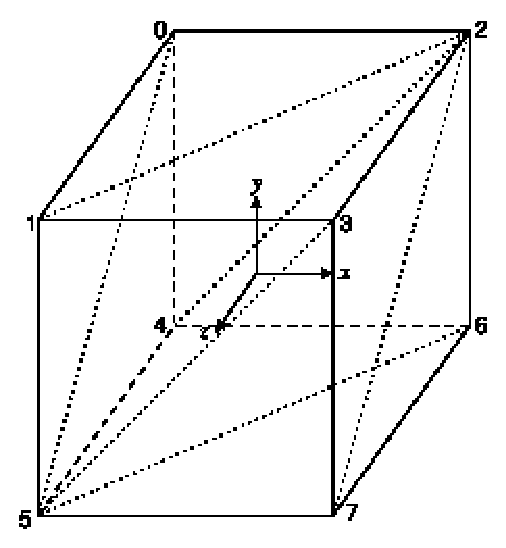
\includegraphics[width=0.2\textwidth]{cube_01}}
 \subfloat[Vertex list.]{
\raisebox{3em}{\begin{tabular}{|c|c|c|c|}
	\cline{2-4}
	\multicolumn{1}{c|}{} & \multicolumn{3}{c|}{\textbf{Vertex List}} \\
	\hline
	\textbf{Vertex ID} & \textbf{x} & \textbf{y} & \textbf{z} \\
	\hline
	0 & -2.5 cm &  2.5 cm & -2.5 cm \\
	\hline
	1 & -2.5 cm &  2.5 cm &  2.5 cm \\
	\hline
	2 &  2.5 cm &  2.5 cm & -2.5 cm \\
	\hline
	3 &  2.5 cm &  2.5 cm &  2.5 cm \\
	\hline
	4 & -2.5 cm & -2.5 cm & -2.5 cm \\
	\hline
	5 & -2.5 cm & -2.5 cm &  2.5 cm \\
	\hline
	6 &  2.5 cm & -2.5 cm & -2.5 cm \\
	\hline
	7 &  2.5 cm & -2.5 cm &  2.5 cm \\
	\hline
\end{tabular}}
 }
\subfloat[Index list.]{
\raisebox{1em}{
\begin{tabular}{|c|c|c|c|}
	\cline{2-4}
	\multicolumn{1}{c|}{} & \multicolumn{3}{c|}{\textbf{Face List}} \\
	\cline{2-4}
	\multicolumn{1}{c|}{} & \textbf{i} & \textbf{j} & \textbf{k} \\
	\hline
	Top face & 1 & 2 & 0 \\
	\hline
	Top face & 2 & 1 & 3 \\
	\hline
	Bottom face & 6 & 5 & 4 \\
	\hline
	Bottom face & 5 & 6 & 7 \\
	\hline
	Front face & 5 & 3 & 1 \\
	\hline
	Front face & 3 & 5 & 7 \\
	\hline
	Back face & 2 & 4 & 0 \\
	\hline
	Back face & 4 & 2 & 6 \\
	\hline
	Left face & 5 & 0 & 4 \\
	\hline
	Left face & 0 & 5 & 1 \\
	\hline
	Right face & 2 & 7 & 6 \\
	\hline
	Right face & 7 & 2 & 3 \\
	\hline
\end{tabular}}}
 \caption{\label{fig:cube_01} Topology of the first cube.}
\end{figure}

\begin{figure}[tbh]
 \centering
 \subfloat[Geometry.]{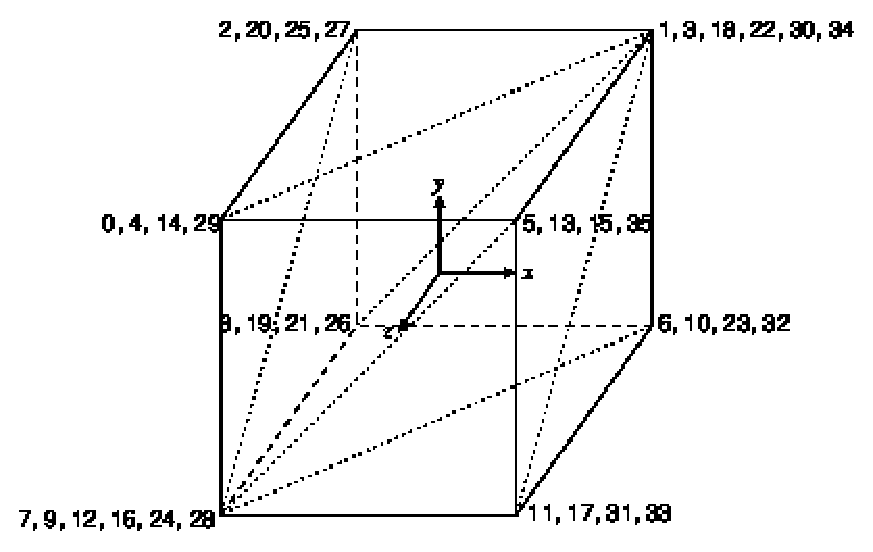
\includegraphics[width=0.35\textwidth]{cube_02}}
\subfloat[Vertex list.]{
\raisebox{2cm}{\begin{tabular}{|c|c|c|c|}
	\cline{2-4}
	\multicolumn{1}{c|}{} & \multicolumn{3}{c|}{\textbf{Vertex List}} \\
	\hline
	\textbf{Vertex ID} & \textbf{x} & \textbf{y} & \textbf{z} \\
	\hline
% 	// Top face
	 0 & -2.5 cm &  2.5 cm & 2.5 cm \\
	\hline
	 1 & 2.5 cm &  2.5 cm & -2.5 cm \\
	\hline
	 $\vdots$ & $\vdots$ & $\vdots$ & $\vdots$ \\
	\hline
% 	 2 & -2.5 cm &  2.5 cm & -2.5 cm \\
% 	\hline
% 	 3 & 2.5 cm &  2.5 cm & -2.5 cm \\
% 	\hline
% 	 4 & -2.5 cm &  2.5 cm & 2.5 cm \\
% 	\hline
% 	 5 & 2.5 cm &  2.5 cm & 2.5 cm \\
% 	\hline
% % 	// Bottom face
% 	 6 & 2.5 cm & -2.5 cm & -2.5 cm \\
% 	\hline
% 	 7 & -2.5 cm & -2.5 cm &  2.5 cm \\
% 	\hline
% 	 8 & -2.5 cm & -2.5 cm & -2.5 cm \\
% 	\hline
% 	 9 & -2.5 cm & -2.5 cm &  2.5 cm \\
% 	\hline
% 	10 & 2.5 cm & -2.5 cm & -2.5 cm \\
% 	\hline
% 	11 &  2.5 cm & -2.5 cm &  2.5 cm \\
% 	\hline
% % 	// Front face
% 	12 & -2.5 cm & -2.5 cm &  2.5 cm \\
% 	\hline
% 	13 & 2.5 cm &  2.5 cm & 2.5 cm \\
% 	\hline
% 	14 & -2.5 cm &  2.5 cm & 2.5 cm \\
% 	\hline
% 	15 & 2.5 cm &  2.5 cm & 2.5 cm \\
% 	\hline
% 	16 & -2.5 cm & -2.5 cm &  2.5 cm \\
% 	\hline
% 	17 &  2.5 cm & -2.5 cm &  2.5 cm \\
% 	\hline
% % 	// Back face
% 	18 & 2.5 cm &  2.5 cm & -2.5 cm \\
% 	\hline
% 	19 & -2.5 cm & -2.5 cm & -2.5 cm \\
% 	\hline
% 	20 & -2.5 cm &  2.5 cm & -2.5 cm \\
% 	\hline
% 	21 & -2.5 cm & -2.5 cm & -2.5 cm \\
% 	\hline
% 	22 & 2.5 cm &  2.5 cm & -2.5 cm \\
% 	\hline
% 	23 & 2.5 cm & -2.5 cm & -2.5 cm \\
% 	\hline
% % 	// Left face
% 	24 & -2.5 cm & -2.5 cm &  2.5 cm \\
% 	\hline
% 	25 & -2.5 cm &  2.5 cm & -2.5 cm \\
% 	\hline
% 	26 & -2.5 cm & -2.5 cm & -2.5 cm \\
% 	\hline
% 	27 & -2.5 cm &  2.5 cm & -2.5 cm \\
% 	\hline
% 	28 & -2.5 cm & -2.5 cm &  2.5 cm \\
% 	\hline
% 	29 & -2.5 cm &  2.5 cm & 2.5 cm \\
% 	\hline
% % 	// Right face
% 	30 & 2.5 cm &  2.5 cm & -2.5 cm \\
% 	\hline
% 	31 &  2.5 cm & -2.5 cm &  2.5 cm \\
% 	\hline
% 	32 & 2.5 cm & -2.5 cm & -2.5 cm \\
% 	\hline
% 	33 &  2.5 cm & -2.5 cm &  2.5 cm \\
% 	\hline
	34 & 2.5 cm &  2.5 cm & -2.5 cm \\
	\hline
	35 & 2.5 cm &  2.5 cm & 2.5 cm \\
	\hline
\end{tabular}}}
 \caption{\label{fig:cube_02} Topology of the second cube.}
\end{figure}

 


\lstinputlisting[firstline=269, lastline=292, caption=Create \Acrshort{3D} 
	objects., label=lst:Load Objects]{../../../examples/src/tutorial_01.cxx}


%%%%%%%%%%%%%%%%%%%%%%%%%%%%%%%%%%%%%%%%%%%%%%%%%%%%%%%%%%%%%%%%%%%%%%%%%%%%%%%%
\section{Display the \Acrshort{3D} Scene}
\label{sec:Display Scene}

Listing~\ref{lst:Display Scene} display the \gls{3D} objects.

\lstinputlisting[firstline=300, lastline=374, caption=display the 
	\Acrshort{3D} scene., label=lst:Display 
	Scene]{../../../examples/src/tutorial_01.cxx}


%%%%%%%%%%%%%%%%%%%%%%%%%%%%%%%%%%%%%%%%%%%%%%%%%%%%%%%%%%%%%%%%%%%%%%%%%%%%%%%%
\section{Idle Callback}
\label{sec:Idle Callback}


\lstinputlisting[firstline=378, lastline=385, caption=Idle callback., 
label=lst:Idle callback]{../../../examples/src/tutorial_01.cxx}

	
%%%%%%%%%%%%%%%%%%%%%%%%%%%%%%%%%%%%%%%%%%%%%%%%%%%%%%%%%%%%%%%%%%%%%%%%%%%%%%%%
\section{Quit Callback}
\label{sec:Quit Callback}


\lstinputlisting[firstline=388, lastline=402, caption=Quit callback., 
label=lst:Quit callback]{../../../examples/src/tutorial_01.cxx}


%%%%%%%%%%%%%%%%%%%%%%%%%%%%%%%%%%%%%%%%%%%%%%%%%%%%%%%%%%%%%%%%%%%%%%%%%%%%%%%%
\section{Frame Buffer Size Callback}
\label{sec:frame buffer callback}


\lstinputlisting[firstline=405, lastline=435, caption=Change of frame buffer 
size callback., 
label=lst:frame buffer callback]{../../../examples/src/tutorial_01.cxx}


%%%%%%%%%%%%%%%%%%%%%%%%%%%%%%%%%%%%%%%%%%%%%%%%%%%%%%%%%%%%%%%%%%%%%%%%%%%%%%%%
\section{Keyboard Callback}
\label{sec:Keyboard Callback}


\lstinputlisting[firstline=438, lastline=456, caption=Keyboard callback., 
label=lst:Keyboard Callback]{../../../examples/src/tutorial_01.cxx}


%%%%%%%%%%%%%%%%%%%%%%%%%%%%%%%%%%%%%%%%%%%%%%%%%%%%%%%%%%%%%%%%%%%%%%%%%%%%%%%%
\section{Scroll Button Callback}
\label{sec:Scroll button callback}


\lstinputlisting[firstline=459, lastline=472, caption=Scroll button callback., 
label=lst:Scroll button callback]{../../../examples/src/tutorial_01.cxx}


%%%%%%%%%%%%%%%%%%%%%%%%%%%%%%%%%%%%%%%%%%%%%%%%%%%%%%%%%%%%%%%%%%%%%%%%%%%%%%%%
\section{Error Callback}
\label{sec:Error Callback}

\lstinputlisting[firstline=475, lastline=481, caption=Error callback., 
label=lst:Error Callback]{../../../examples/src/tutorial_01.cxx}



\section{Next Tutorial...}

In the next tutorial:
\begin{itemize}
	\item Load the shader from a file compressed using 
		the Zlib\,\footnote{\url{http://www.zlib.net/}}
%  \item  You will see how to get rid of OpenGL's fixed pipeline (which is now depreciated). 
%  
%  \item You will see how to get rid of OpenGL's matrix stack (which is now depreciated).
% 
	\item We will see how to create an efficient mouse control to turn the 
		\Acrshort{3D} scene. 
% 
%  \item You will also see how to update the topology of the triangle meshes. 
%  This is important in medical simulations with soft tissue deformations. 
\end{itemize}


% \newpage
\ifpdf
\printglossary[type=\acronymtype] 
\fi

\appendix
\section{Program Source Code}
\label{sec:Program Source Code}

\lstinputlisting[caption=All the source code of this tutorial., 
label=lst:Program Source Code]{../../../examples/src/tutorial_01.cxx}

% 
% \newpage
% \phantomsection
% \addcontentsline{toc}{section}{References}
% \printbibliography
% 

\end{document}
